\documentclass[11pt]{beamer}
\usetheme{Warsaw}
\usepackage[utf8]{inputenc}
\usepackage{amsmath}
\usepackage{amsfonts}
\usepackage{amssymb}

\author{Jauntyliu @ SCGY-Tech}
\title{Lessons on Linux, Server and Git}
%\setbeamercovered{transparent} 
%\setbeamertemplate{navigation symbols}{} 
%\logo{} 
%\institute{} 
%\date{} 
%\subject{} 

\begin{document}

\begin{frame}
\titlepage
\end{frame}

%\begin{frame}
%\tableofcontents
%\end{frame}

\begin{frame}
\frametitle{What is Linux?}

Linux:
\begin{itemize}
\item an operating system kernel written by Linus Torvalds in 1991
\item components of the most famous open-source operating system
\item highly scalable, customizable and stable
\item distributes along with many free software
\item full source code available at \href{http://www.kernel.org}{kernel.org}
\end{itemize}

\end{frame}



\begin{frame}
\frametitle{Linux Distributions}
Linux itself is just a kernel. Without various applications, the OS wouldn't be usable.

A combination of Linux (the kernel) and its applications formed a \textbf{distribution}.
\begin{itemize}
\item Ubuntu
\item Debian
\item Fedora
\item RHEL \& CentOS
\item Arch Linux
\item Gentoo \& Linux From Scratch
\item Slax, Kali, Deepin, Tiny Core Linux...
\end{itemize}
\end{frame}

\begin{frame}
\frametitle{OSS License}
In open-source software, the freedom of users is guaranteed by software licenses.
\begin{itemize}
\item GNU General Public License
\item GNU Lesser General Public License
\item Apache \& MIT \& BSD License
\item ...
\end{itemize}
\end{frame}

\begin{frame}
\frametitle{Basic Environment Setup}
Today, I'll share my Raspberry Pi 3B+ as a Linux host with you to enjoy.
To connect:
\begin{enumerate}
\item Download PuTTY from \href{http://home.ustc.edu.cn/~jauntyliu/}{my homepage}
\item Extract and run PUTTY.EXE, fill the Host Name field with \textbf{192.168.2.141}
\item Type \textbf{tempuser} as "\textit{Login as:}" appears
\item Type \textbf{233} as "\textit{Password:}" appears.

\textbf{Notice:} the password you type \textbf{will not be shown} on screen as Unix tradition
%\item Type the account name and password you desired.
%\item Close yout PuTTY session, reopen it, type the same Host Name
%\item This time type the account and password you registered just now.createaccount



\end{enumerate}
\end{frame}

\begin{frame}
\frametitle{Basic Shell Commands}
Format:
\textbf{path\_to\_executable} \textit{argument0} \textbf{argument1} $\cdots$

Example:
\begin{itemize}
\item cp a.txt b.txt

Here, \textbf{cp} is the shorthand of \textbf{/usr/bin/cp}, and \textbf{a.txt} is the first argument, \textbf{b.txt} the second.
\item ls

A program can run without any arguments given.
\end{itemize}
\end{frame}

\begin{frame}
\frametitle{Unix Paths}
The Unix paths consists of two types:
\begin{enumerate}
\item Absolute Path :  Always start with /
\begin{itemize}
\item (a folder)\textbf{/usr/bin} 
\item  (a file)\textbf{/usr/bin/ls}
\end{itemize}
Unlike disk C: and D: in Windows, there is only a single \textbf{Root} (/) in Linux, and real drives are mounted as folders of the root filesystem.

\item Relative Path: A \textbf{part} of the path, only useful when given the \textbf{current working directory}.\\
Suppose you're in \textbf{/usr} (a folder)
\begin{itemize}
\item \textbf{bin/ls} - the same as /usr/bin/ls
\item \textbf{.} - the dots means "\textit{current directory}", hence "\textbf{/usr/}" itself
\item \textbf{..} - the double dots means "\textit{parent directory}", hence "\textbf{/}"
\item \textbf{../home/../dev/../usr} - also means \textbf{/usr} 
\end{itemize}
\end{enumerate}
\end{frame}

\begin{frame}
\frametitle{Basic Shell Commands}
\begin{itemize}
\item ls - \textbf{list directories}
\item cd - \textbf{change directory}
\item pwd - \textbf{print working directory}
\item mv - \textbf{move file}
\item cp - \textbf{copy file}
\item rm - \textbf{remove file}
\item mkdir - \textbf{create a directory}
\item man - \textbf{manual pages}
\item apropos - \textbf{looking for relative commands and programs}
\end{itemize}

Mission 1: Create a directory called "\textbf{XcxSaikou}" in your home directory  and copy \textbf{/etc/apt/sources.list} into the folder you create.
\end{frame}

\begin{frame}
\frametitle{Basic Shell Commands}
How to get help?
\begin{enumerate}
\item \textbf{the\_commands\_you\_don't\_understand --help}
\item \textbf{man the\_commands\_you\_don't\_understand}
\item \textbf{apropos the\_keyword\_about\_what\_you\_want}
\item Google \& Stack Overflow
\item Ask in SCGY-Tech or USTCLUG
\end{enumerate}
\end{frame}

\begin{frame}
\frametitle{Basic Shell Commands}
One possible solution:
\begin{enumerate}
\item mkdir ~/XcxSaikou
\item cp /etc/apt/source.list ~/XcxSaikou
\item cd ~/XcxSaikou
\item ls -l
\end{enumerate}
\end{frame}


\begin{frame}
\frametitle{What's under \textbf{/}?}
Mission 2: Find what's under "\textbf{/}"?
\end{frame}

\begin{frame}
\frametitle{What's under \textbf{/}?}
\begin{itemize}
\item \textbf{/home} - User home directories\\
In Unix, the directory \textbf{/home/your\_account} is the most decent place for you to store your personal data.
\item \textbf{/usr} - Executables, libraries, and shared resources that are not system critical
\item \textbf{/etc} - System-wide configuration files and system databases
\item \textbf{/dev} - Devices, such as hard disks, ttys and displays.
\item \textbf{/var} - Log files, print jobs, mails and temporaries
\item \textbf{/lib} - Shared libraries, kernel module or device drivers.
\item \textbf{/bin} - Binaries that should be available even when \textbf{/usr} haven't been mounted
\item $\cdots$
\end{itemize}
\end{frame}

\begin{frame}
\frametitle{Basic File Editing}
\begin{itemize}
\item User-friendly: \textbf{nano a.txt}
\item Experienced: \textbf{vim a.txt}
\item Obsolete: \textbf{ed a.txt}
\end{itemize}
Mission 3: Create a text file called "\textbf{Comments\_On\_Fruits.txt}" and write some words in it. You may use any of them if you like.
\end{frame}

\begin{frame}
\frametitle{Users and Permissions}
Users are entities who operate on this system.
\begin{itemize}
\item Every file and folder has an owner
\item Users can only Read/Write/eXecute when they have the permission
\item Use \textbf{ls -l} to see the permissions:\\
\end{itemize}
\begin{tabular}{llllll}
-rw-r--r-- & 1 & libreliu & sudo  &        38 Oct 15 23:29 & flag.txt\\
drwxr-xr-x &  5  & libreliu & sudo &       4096 Oct 18 20:37 & writeup\\
\end{tabular}


\end{frame}

\begin{frame}
\begin{figure}
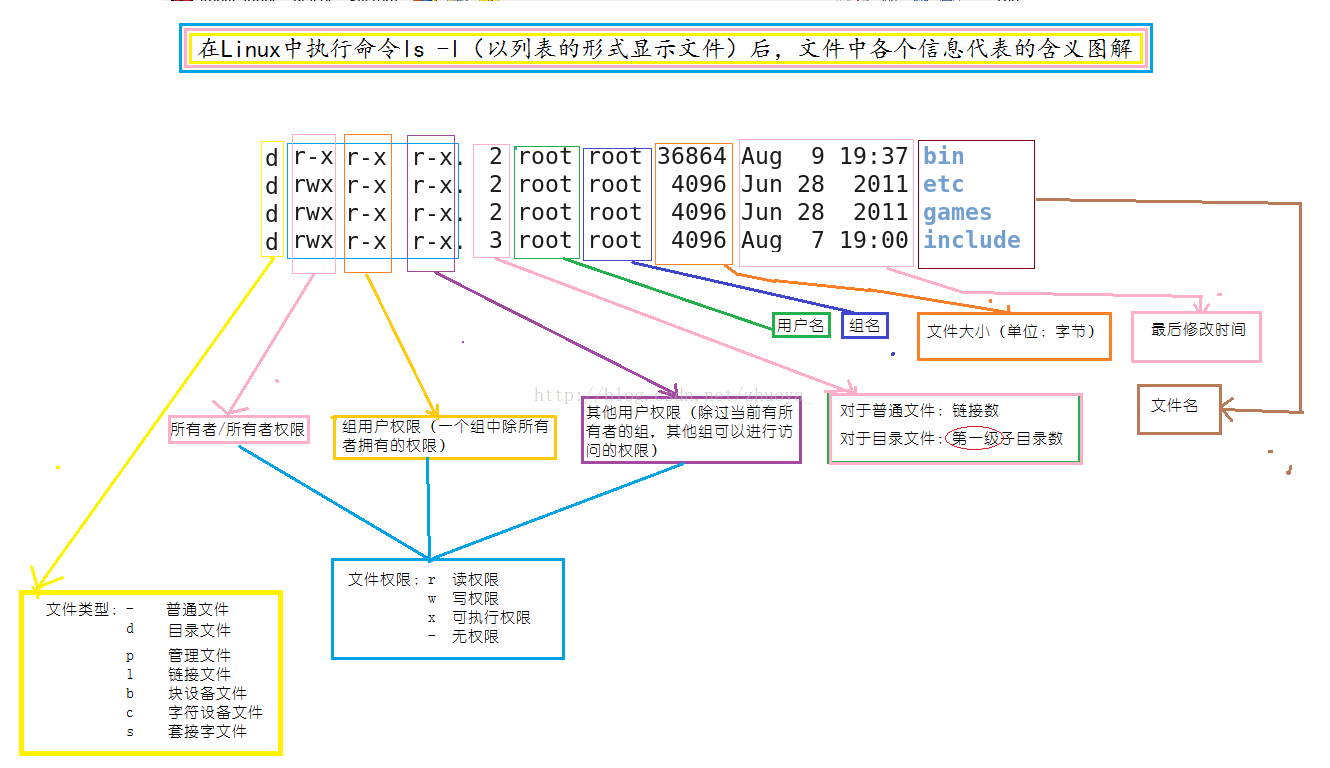
\includegraphics[width=\textwidth]{ls_description.png}
%\includegraphics [width=3in] {file.eps} 
%将 file.eps 插入文档并且它的宽度被缩放到 3 英寸,高度也会 按相应的比例缩放。
%如果用 \textwidth 或 \em 等的函数来 指定宽度,而不是用像 3 英寸这样的固定尺寸,将会使你的 LATEX 文 档更具通用性。
%例如: \includegraphics [width=\textwidth] {graphics.eps} 
%将所插入图形缩放到和文本行的宽度一样宽。
%而下面的命令 
%\includegraphics [width=0.80\textwidth]{graphics.eps} 
%使得插入图形的宽度为文本行宽的 80%。
%当与 calc 宏包配合使用 时,下面的命令可令图形的宽度比文本行宽少 2 英寸: 
%\includegraphics [width=\textwidth-2.0in]{graphics.eps}
%---------------------
%原文:https://blog.csdn.net/sinat_36301420/article/details/79334728 
\end{figure}
\end{frame}


\begin{frame}
\frametitle{Users and permissions}
Edit file permissions:
\begin{itemize}
\item \textbf{chmod three\_octal\_digits filename} - change permission bits
\item \textbf{chown owner\_name filename} - change file and directory owner\\
Notice: changing the directory along \textbf{WON'T} affect its subdirectories and files.
\end{itemize}
Edit users and their passwords:
\begin{itemize}
\item \textbf{useradd} - add user to the system
\item \textbf{userdel} - delete user
\item \textbf{usermod} - modify user
\item \textbf{passwd} - change user password
\item \textbf{groupadd} - user groups related operations
\end{itemize}
\end{frame}



\begin{frame}[fragile]
\frametitle{Mount and umount in Unix}
\begin{itemize}
\item A storage device must be mounted first before it's available for use. \textbf{At the system's perspective, it needs to know which folder the files of the disk should be in.}
\item \textbf{lsblk} - list block devices, for you to see if your storage device is recognized by the system
\begin{verbatim}
NAME   MAJ:MIN RM   SIZE RO TYPE MOUNTPOINT
sda      8:0    0 298.1G  0 disk 
|-sda1   8:1    0   487M  0 part /boot
|-sda2   8:2    0     1K  0 part 
|-sda5   8:5    0  18.6G  0 part /
|-sda6   8:6    0  74.5G  0 part /home
`-sda7   8:7    0   2.8G  0 part [SWAP]
\end{verbatim}
\item \textbf{mount [-fnrsvw] [-t fstype] [-o options] device dir} - mount a device to a exist empty dir
\end{itemize}
\end{frame}

\begin{frame}
\frametitle{Mount and umount in Unix}
\begin{itemize}
\item \textbf{umount directory} or \textbf{umount device} - detaches the mentioned file system(s) from the file hierarchy
\end{itemize}
\end{frame}

\begin{frame}
\frametitle{Programming under Linux}
Programming under Linux boasts great efficiency
\begin{enumerate}
\item \textbf{sudo apt install build-essential} - Install gcc, make, g++ and so on.
\item \textbf{nano hello.c} - Write C Programs
\item \textbf{gcc hello.c -o hello \&\& ./hello} - Compile and run the program\\
\textbf{\&\&} is just a way to execute two shell commands in a row, just like \textbf{if(c=1 \&\& b=1 \&\& a!=3)} in C
\end{enumerate}
When in doubt
\begin{itemize}
\item \textbf{man 3 printf} - Check for manual pages about library function (section 3) \textbf{printf}
\end{itemize}
\end{frame}

\begin{frame}
\frametitle{Installing software}
For simple software like Browsers and Games:
\begin{enumerate}
\item Use Package Manager, search for it and then install the package (Described later)
\item Build from source: \textbf{./configure \&\& make \&\& sudo make install}
\item When bumping into dependency problems, try installing the missing software
\item When you've tried everything, discuss with others or open an issue to the project (forum) directly
\end{enumerate}

For complicated, highly configurable software:
\begin{enumerate}
\item Looking for things like "\textbf{How to install and configure xxx}" on the Internet
\item Follow the instructions
\end{enumerate}

Homework: Try building \textbf{nginx} web server from source.
\end{frame}


\begin{frame}
\frametitle{Package Manager}
Package manager helps you install software easily, without having to solve dependencies on your own, as well as upgrading the software by hand
\begin{itemize}
\item apt for Debian/Ubuntu
\item yum \& rpm for Fedora/OpenSUSE/CentOS/RHEL
\item pacman for Arch Linux
\end{itemize}
They share some similar traits:
\begin{itemize}
\item Configurations for Software Sources - Integrated database for software packages\\
See \textit{\href{http://mirrors.ustc.edu.cn}{USTCLUG Mirrors}}
\item \textbf{apt install software\_name}
\item \textbf{pacman -S software\_name}
\item See manpages for more details
\end{itemize}
\end{frame}

\begin{frame}
\frametitle{SSH Operations}
SSH stands for \textit{Secure Shell}, a software suite and a protocol designed for delivering remote shell, file copying and port-forwarding.
\begin{itemize}
\item \textbf{ssh tempuser@192.168.4.233} - initiate a connection to remote machine, with username tempuser.\\
When username was not specified, the ssh client will attempts to connect with local username that's using.
\item \textbf{scp -r tempuser@192.168.4.233:/home/tempuser /home/tempuser/archive\_at\_remote} - copy files from remote machine by using \textit{Secure Copy} command
\end{itemize}

Mission 4: Try copying files \textbf{flag.txt} from my laptop by using the account I given.
\end{frame}

\begin{frame}
\frametitle{Git and Github}


\end{frame}



\end{document}